\documentclass{beamer}

\usepackage[utf8]{inputenc}
\usepackage[spanish]{babel}
\usepackage{amsmath}
\usepackage[nosetup]{evan}
\usetheme{Madrid}
%\usetheme{Goddard}
\hypersetup{colorlinks,allcolors=.,urlcolor=magenta}
\usepackage[table]{xcolor} % Para definir colores en tablas
\usepackage{graphicx} % Para redimensionar la tabla
\usepackage{multicol}

\title{Investigación de Operaciones I}
\subtitle{Unidad 2: Aspectos de Dualidad y Análisis de Sensibilidad}
\author[Ricardo Largaespada]{Ricardo Jesús Largaespada Fernández}
\institute[UNI]{Ingeniería de Sistemas, DACTIC, UNI}
\date{14 de Octubre, 2024}

\begin{document}

\frame{\titlepage}

\begin{frame}
\frametitle{Agenda}
\tableofcontents
\end{frame}

\section{Interpretación económica de la Dualidad}
\begin{frame}
\frametitle{Interpretación económica de la Dualidad.}
\begin{itemize}
\item Interpretación de las restricciones duales.\\
\item Interpretación de las variables duales.
\end{itemize}
\pause
\textbf{Objetivos de Aprendizaje}
    \begin{enumerate}
        \item Comprender y explicar la importancia de las restricciones duales en la interpretación económica de la dualidad, identificando cómo influyen en la optimización de un problema económico.
        \item Analizar y relacionar las variables duales con la interpretación económica de la dualidad, identificando su papel en la formulación y resolución de problemas económicos.
    \end{enumerate}
\end{frame}

\begin{frame}{Un problema de mezcla de productos}
    \begin{itemize}
        \item Supongamos que producimos mesas y sillas utilizando madera y horas de trabajo. En total, contamos con seis unidades de madera y seis horas laborales.
        \begin{itemize}
            \item Cada mesa se vende por $3 y$ requiere 2 unidades de madera y 1 hora de trabajo.
            \item Cada silla se vende por $1$ y requiere 1 unidad de madera y 2 horas de trabajo.
        \end{itemize}
    \end{itemize}
\pause    
    \(x_1\) : número de mesas producidas. \(x_2\) : número de sillas producidas.\\
\begin{multicols}{2}
    \textbf{La formulación es}:
    \[
    \text{maximizar } \quad 3x_1 + x_2
    \]
    \text{Sujetos a:}
    \[
    2x_1 + x_2 \leq 6
    \]
    \[
    x_1 + 2x_2 \leq 6
    \]
    \[
    x_i \geq 0 \quad \forall i = 1, 2.
    \]
    
    \textbf{La solución óptima es:} $x^* = (3,0)$.
    \begin{center}
        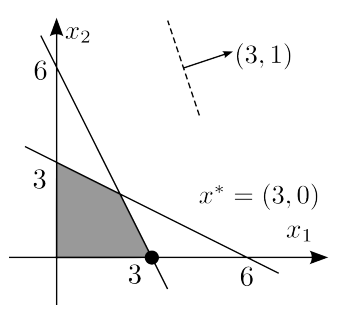
\includegraphics[scale=.5]{images/shadows1.png}
    \end{center}
\end{multicols}
\end{frame}

\begin{frame}{Preguntas de “¿Qué pasaría si?”}
    \begin{itemize}
        \item En la práctica, las personas a menudo hacen preguntas de “¿qué pasaría si?”:
        \begin{itemize}
            \item ¿Qué pasaría si el precio unitario de las sillas se vuelve $2$?
            \item ¿Qué pasaría si cada mesa requiere 3 unidades de madera?
            \item ¿Qué pasaría si tenemos 10 unidades de madera?
        \end{itemize}
    \end{itemize}
\pause
    \begin{itemize}
        \item ¿Por qué hacer preguntas de “¿qué pasaría si?”?
        \begin{itemize}
            \item Los parámetros pueden fluctuar.
            \item La estimación de parámetros puede ser inexacta.
            \item Se buscan maneras de mejorar el negocio.
        \end{itemize}
    \end{itemize}
\pause
    \begin{itemize}
        \item Para problemas realistas, las preguntas de “¿qué pasaría si?” pueden ser complicadas.
        \begin{itemize}
            \item Aun si solo es una modificación pequeña de un parámetro, la solución óptima podría cambiar mucho.
        \end{itemize}
    \end{itemize}
\pause
    \begin{itemize}
        \item La herramienta para responder preguntas de “¿qué pasaría si?” es el \textbf{análisis de sensibilidad}.
    \end{itemize}
\end{frame}

\begin{frame}{Humboldt Redwood}
    \begin{itemize}
        \item La compañía Pacific Lumber (ahora Humboldt Redwood) tiene más de 200,000 acres de bosques y cinco aserraderos.
    \end{itemize}
    
    \begin{itemize}
        \item \textbf{La sostenibilidad} es importante para la toma de decisiones operativas.
        \begin{itemize}
            \item Un equipo de IO desarrolló un plan de gestión de ecosistemas forestales a 120 años.
            \item El PL optimiza las operaciones forestales para maximizar la rentabilidad mientras satisface restricciones, incluyendo sostenibilidad.
            \item El modelo tiene alrededor de 8,500 restricciones funcionales y 353,000 variables.
        \end{itemize}
    \end{itemize}
    
    \begin{itemize}
        \item ¡El entorno puede \textbf{cambiar}!
        \begin{itemize}
            \item Por ejemplo, clima, oferta y demanda, costos de tala y regulaciones.
            \item Se aplica análisis de sensibilidad.
        \end{itemize}
    \end{itemize}
    
    \vspace{1cm}
    \footnotesize{
        \begin{quote}
            L. R. Fletcher, H. Alden, S. P. Holmen, D. P. Angelides, y M. J. Etzenhouser (1999). “Long-term forest ecosystem planning at Pacific Lumber.”. \textit{Interface} 29(1) 90-111. \url{http://dx.doi.org/10.1287/inte.29.1.90}
        \end{quote}
    }
\end{frame}

\begin{frame}{Preguntas de “¿Qué pasaría si?”}
    \begin{itemize}
        \item En general, las preguntas de “¿qué pasaría si?” siempre pueden ser respondidas formulando y resolviendo un nuevo problema de optimización \textbf{desde cero}.
    \end{itemize}

    \begin{itemize}
        \item ¡Pero esto puede ser demasiado lento!
    \end{itemize}

    \begin{itemize}
        \item Con técnicas de análisis de sensibilidad:
        \begin{itemize}
            \item La tabla óptima original proporciona información útil.
            \item Normalmente comenzamos desde la solución básica factible original y realizamos solo \textbf{unas pocas} iteraciones para alcanzar la nueva solución óptima.
            \item La dualidad proporciona un fundamento teórico.
        \end{itemize}
    \end{itemize}
    
    \begin{itemize}
        \item Aquí queremos introducir un tipo de pregunta de “¿qué pasaría si?”: ¿Qué sucede si tengo \textbf{unidades adicionales de un recurso}?
    \end{itemize}

    \begin{itemize}
        \item Consideremos el siguiente escenario:
        \begin{itemize}
            \item Un día, un vendedor llega a tu oficina y quiere ofrecerte una unidad adicional de madera a $1$. ¿Deberías aceptarla o rechazarla?
        \end{itemize}
    \end{itemize}
\end{frame}

\begin{frame}{Una unidad más de madera}
\begin{multicols}{2}
    \begin{itemize}
        \item Para responder a esta pregunta, se puede formular un nuevo PL:
        \[
        \text{maximizar } \quad 3x_1 + x_2
        \]
        \text{Sujetos a:}
        \[
        2x_1 + x_2 \leq 7
        \]
        \[
        x_1 + 2x_2 \leq 6
        \]
        \[
        x_i \geq 0 \quad \forall i = 1, 2.
        \]
    \end{itemize}
    
    \begin{itemize}
        \item El nuevo valor del objetivo:
        \[
        z' = 3 \times 3.5 + 0 = 10.5
        \]
        es mayor que el valor del objetivo anterior $z^* = 9$.
    \end{itemize}

    \begin{itemize}
        \item Es recomendable aceptar la oferta (al precio unitario de $1$).
        \begin{itemize}
            \item Ganamos $0.5$ como nuestro \textbf{beneficio neto}.
        \end{itemize}
    \end{itemize}
\begin{center}
    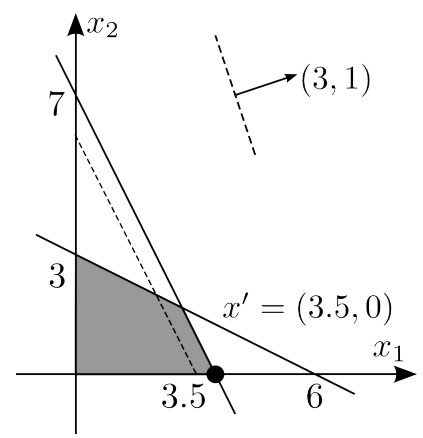
\includegraphics[scale=0.5]{images/shadows2.png}
\end{center}
\end{multicols}
\end{frame}

\begin{frame}{Una hora adicional de trabajo}
\begin{multicols}{2}
    \begin{itemize}
        \item Supongamos que en lugar de ofrecer una unidad adicional de madera, el vendedor ofrece una hora adicional de trabajo a $1$.
    \end{itemize}

    \begin{itemize}
        \item La nueva formulación del problema es:
        \[
        \text{maximizar } \quad 3x_1 + x_2
        \]
        \text{Sujetos a:}
        \[
        2x_1 + x_2 \leq 6
        \]
        \[
        x_1 + 2x_2 \leq 7
        \]
        \[
        x_i \geq 0 \quad \forall i = 1, 2.
        \]
    \end{itemize}

    \begin{itemize}
        \item El nuevo valor del objetivo es \textbf{el mismo} que el valor del objetivo anterior.
    \end{itemize}

    \begin{itemize}
        \item No es rentable comprarla: El valor objetivo no aumenta.
        \begin{itemize}
            \item La \textbf{pérdida neta} es de $1$.
        \end{itemize}
    \end{itemize}
    \begin{center}
        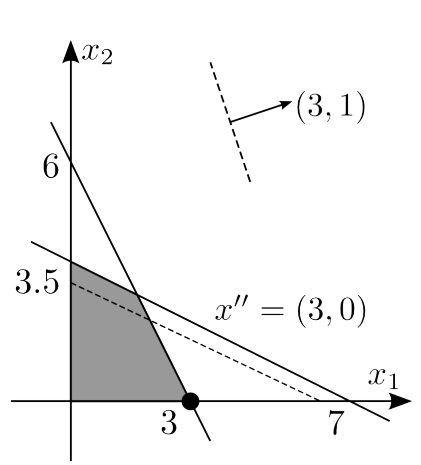
\includegraphics[scale=0.5]{images/shadows3.png}
    \end{center}
\end{multicols}
\end{frame}

\begin{frame}{Precios sombra}
    \begin{itemize}
        \item Para cada recurso, existe un \textbf{precio máximo} que estamos dispuestos a pagar por una unidad adicional.
        \begin{itemize}
            \item Esto depende del beneficio neto de esa unidad adicional.
            \item Para la madera, este precio es de $1.5$. Para las horas laborales, este precio es de $0$.
        \end{itemize}
    \end{itemize}

    \begin{itemize}
        \item Esto nos motiva a definir los \textbf{precios sombra} para cada restricción:
    \end{itemize}
    
    \begin{block}{Definición 1 (Precio sombra)}
        Para un PL que tiene una solución óptima, el precio sombra de una restricción es la cantidad en que aumenta el valor del objetivo cuando el lado derecho de esa restricción aumenta en 1, asumiendo que la base óptima actual permanece óptima.
    \end{block}
    
    \begin{itemize}
        \item Entonces, para nuestro ejemplo de mesa-silla, los precios sombra de las restricciones 1 y 2 son 1.5 y 0, respectivamente.
    \end{itemize}
    
    \begin{itemize}
        \item Nota que asumimos que la base óptima actual no cambia.
    \end{itemize}
\end{frame}

\begin{frame}{Asumiendo que la base óptima no cambia}
\begin{columns}
  \begin{column}{0.6\textwidth}
  {\tiny 
    \begin{itemize}
        \item Consideremos otro ejemplo:
        \[
        z^* = \text{maximizar } \quad 3x_1 + x_2
        \]
        \text{Sujetos a:}
        \[
        x_1 + x_2 \leq 4
        \]
        \[
        x_1 + 2x_2 \leq 4.5
        \]
        \[
        x_i \geq 0 \quad \forall i = 1, 2.
        \]
    \end{itemize}
    
    \begin{itemize}
        \item Si queremos encontrar el precio sombra de la restricción 1, podemos intentar resolver un nuevo PL:
        \[
        z^{**} = \text{maximizar } \quad 3x_1 + x_2
        \]
        \text{Sujetos a:}
        \[
        x_1 + x_2 \leq 5
        \]
        \[
        x_1 + 2x_2 \leq 4.5
        \]
        \[
        x_i \geq 0 \quad \forall i = 1, 2.
        \]
    \end{itemize}

    \begin{itemize}
        \item Aunque $z^{**} = 13.5$ y $z^* = 12$, el precio sombra es $15 - 12 = 3$, \textbf{no 1.5}
    \end{itemize}
    
    \begin{itemize}
        \item Los precios sombra miden la \textbf{tasa} de mejora.
    \end{itemize}
    }
  \end{column}
  \begin{column}{0.4\textwidth}
    % Imagen a la derecha
    \centering
    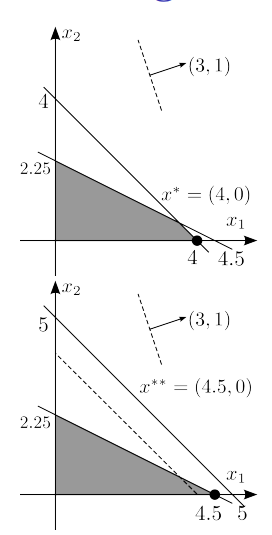
\includegraphics[width=0.75\textwidth]{images/shadows4.png}
  \end{column}
\end{columns}
\end{frame}

\begin{frame}{Signos de los precios sombra}
    \begin{itemize}
        \item Dado que un precio sombra mide cómo se incrementa el valor del objetivo, su signo se determina en base a cómo cambia la región factible:
    \end{itemize}
    
    \begin{block}{Signos de los precios sombra}
        Para cualquier PL, el signo de un precio sombra sigue la regla indicada a continuación:
        
        \begin{center}
            \begin{tabular}{|c|c|c|c|}
                \hline
                \textbf{Función objetivo} & \(\leq\) & \(\geq\) & \(=\) \\
                \hline
                \text{max} & \(\geq 0\) & \(\leq 0\) & \text{Libre} \\
                \text{min} & \(\leq 0\) & \(\geq 0\) & \text{Libre} \\
                \hline
            \end{tabular}
        \end{center}
    \end{block}
\end{frame}

\begin{frame}{Precios sombra de restricciones no vinculantes}
    \begin{itemize}
        \item Si al modificar una restricción no se afecta la solución óptima, el precio sombra debe ser \textbf{cero}.${}^{4}$
    \end{itemize}
    
    \begin{block}{}
        Los precios sombra son cero para las restricciones que no son vinculantes en la solución óptima.
    \end{block}

    \begin{itemize}
        \item Ahora sabemos que encontrar los precios sombra nos permite responder preguntas relacionadas con unidades adicionales de recursos.
    \end{itemize}

    \begin{itemize}
        \item Pero, ¿cómo encontrar \textbf{todos} los precios sombra?
        \begin{itemize}
            \item Sea \( m \) el número de restricciones.
            \item ¿Existe una mejor manera que resolver \( m \) problemas lineales?
            \item ¡La dualidad ayuda!
        \end{itemize}
    \end{itemize}
    
    \vspace{0.5cm}
    \footnotesize{
        \begin{quote}
            ${}^{4}$No todas las restricciones vinculantes tienen precios sombra distintos de cero. ¿Por qué?
        \end{quote}
    }
\end{frame}

\begin{frame}{La solución óptima dual proporciona precios sombra}
    \begin{block}{}
        Para cualquier PL, los precios sombra son iguales a los valores de las variables duales en la solución óptima dual.
    \end{block}

    \begin{itemize}
        \item \textbf{Prueba.} Sea \( B \) la base óptima antigua y \( z = c_B^T A_B^{-1} b \) el valor objetivo antiguo. Si \( b_1 \) se convierte en \( b_1' = b_1 + 1 \), entonces \( z \) se convierte en:
    \end{itemize}
    
    \[
    z' = c_B^T A_B^{-1} \left( b + 
    \begin{bmatrix}
        1 \\
        0 \\
        \vdots \\
        0
    \end{bmatrix} \right) 
    = z + \left( c_B^T A_B^{-1} \right)_1.
    \]

    \begin{itemize}
        \item Por lo tanto, el precio sombra de la restricción 1 es \( \left( c_B^T A_B^{-1} \right)_1 \). En general, el precio sombra de la restricción \( i \) es \( \left( c_B^T A_B^{-1} \right)_i \). Como \( c_B^T A_B^{-1} \) es la solución óptima dual, la prueba está completa.
    \end{itemize}
    
    \begin{flushright}
        \(\square\)
    \end{flushright}
\end{frame}

\begin{frame}{Un ejemplo}
\begin{columns}
\begin{column}{0.6\textwidth}
{\tiny 
\begin{itemize}
        \item ¿Cuáles son los precios sombra?
        \[
        \text{minimizar } \quad 6x_1 + 4x_2
        \]
        \text{Sujetos a:}
        \[
        x_1 + x_2 \geq 2
        \]
        \[
        3x_1 + x_2 \geq 1
        \]
        \[
        x_i \geq 0 \quad \forall i = 1, 2.
        \]
    \end{itemize}
    
    \begin{itemize}
        \item Resolvemos el PL dual:
        \[
        \text{maximizar } \quad 2y_1 + y_2
        \]
        \text{Sujetos a:}
        \[
        y_1 + 3y_2 \leq 6
        \]
        \[
        y_1 + y_2 \leq 4
        \]
        \[
        y_i \geq 0 \quad \forall i = 1, 2.
        \]
    \end{itemize}
    
    \begin{itemize}
        \item La solución óptima dual es \( y^* = (4, 0) \).
    \end{itemize}
    
    \begin{itemize}
        \item Entonces, los precios sombra son 4 y 0, respectivamente.
    \end{itemize}}
\end{column}
\begin{column}{0.4\textwidth}
    \begin{center}
        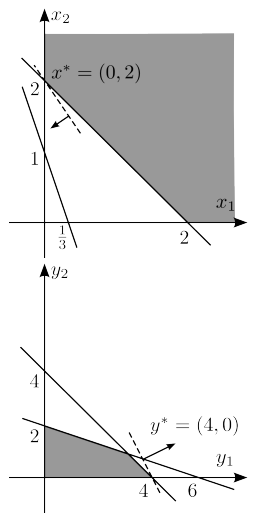
\includegraphics[width=0.75\textwidth]{images/shadows5.png}
    \end{center}
\end{column}
\end{columns}
\end{frame}

% Diapositiva 1: Introducción a las Restricciones Duales
\begin{frame}{Introducción a las Restricciones Duales}
    \begin{itemize}
        \item \textbf{Definición:} Las restricciones duales se derivan de las variables duales o precios sombra, que reflejan el valor adicional que se puede obtener al incrementar un recurso correspondiente.
        \item \textbf{Concepto de dualidad:} Relación entre el problema primal y el dual que permite analizar la sensibilidad de las restricciones.
        \item \textbf{Importancia:} Permiten identificar el uso óptimo de los recursos y evaluar decisiones estratégicas en un problema económico.
    \end{itemize}
\end{frame}

% Diapositiva 2: Interpretación Económica
\begin{frame}{Interpretación Económica}
    \begin{itemize}
        \item Los precios sombra indican el \textbf{valor marginal} de los recursos limitados.
        \item Si el precio sombra es positivo, se justifica económicamente obtener más de ese recurso.
        \item Si el precio sombra es cero o negativo, no es rentable adquirir más de ese recurso.
        \item Ejemplo: En un problema de producción, el precio sombra de un recurso como mano de obra indica cuánto aumenta el beneficio total si se dispone de una hora adicional de trabajo.
    \end{itemize}
\end{frame}

% Diapositiva 3: Influencia en la Optimización
\begin{frame}{Influencia en la Optimización}
    \begin{itemize}
        \item \textbf{Identificación de restricciones críticas:} Aquellas con precio sombra positivo.
        \item \textbf{Identificación de restricciones no críticas:} Aquellas con precio sombra cero.
        \item Una restricción crítica indica que el recurso correspondiente se usa en su capacidad máxima.
        \item Una restricción no crítica sugiere que hay capacidad no utilizada.
    \end{itemize}
\end{frame}

% Diapositiva 4: Importancia en la Toma de Decisiones
\begin{frame}{Importancia en la Toma de Decisiones}
    \begin{itemize}
        \item Los precios sombra proporcionan información para:
        \begin{itemize}
            \item Aumentar o disminuir la oferta de un recurso.
            \item Redefinir las políticas de producción para mejorar la eficiencia.
            \item Estimar el impacto económico de los cambios en la disponibilidad de recursos.
        \end{itemize}
        \pause
        \item Permiten evaluar el \textbf{beneficio neto} de cada recurso adicional en un problema económico.
    \end{itemize}
\end{frame}

% Diapositiva 5: Ejercicio Práctico
\begin{frame}{Ejercicio Práctico}
    \textbf{Contexto:} Una empresa agrícola produce maíz y trigo. Tiene 200 horas de trabajo y 150 toneladas de fertilizantes. El objetivo es maximizar las ganancias dadas las siguientes restricciones:
    \begin{itemize}
        \item \textbf{Maíz:} 50 horas de trabajo y 30 toneladas de fertilizantes por tonelada producida.
        \item \textbf{Trigo:} 40 horas de trabajo y 20 toneladas de fertilizantes por tonelada producida.
        \item \textbf{Ganancias:} Maíz $= 200$ USD/ton, Trigo $= 150$ USD/ton.
    \end{itemize}
    \textbf{Preguntas:}
    \begin{enumerate}
        \item ¿Cuáles son las restricciones duales del problema?
        \item Identificar y calcular los precios sombra de cada recurso.
        \item Explicar el significado económico de los precios sombra.
        \item ¿Cuál recurso debería adquirir la empresa para maximizar sus beneficios?
    \end{enumerate}
\end{frame}

% Diapositiva 6: Análisis de Casos Reales
\begin{frame}{Análisis de Casos Reales}
    \textbf{Caso 1: Asignación de Recursos en el Sector Salud}
    \begin{itemize}
        \item Un hospital debe asignar médicos y equipos limitados a diferentes áreas.
        \item Los precios sombra permiten identificar áreas críticas y ajustar la distribución de recursos.
        \item Resultado: Se optimiza la calidad del servicio sin aumentar costos.
    \end{itemize}
\end{frame}

% Diapositiva 7: Caso 2 - Producción en el Sector Automotriz
\begin{frame}{Caso 2: Producción en el Sector Automotriz}
    \begin{itemize}
        \item Una empresa automotriz produce vehículos con restricciones de acero y mano de obra.
        \item Se determina que el acero es crítico (precio sombra alto) y la mano de obra es no crítica.
        \item Resultado: La empresa invierte en nuevas fuentes de acero para optimizar su producción.
    \end{itemize}
\end{frame}

% Diapositiva 8: Caso 3 - Política Monetaria
\begin{frame}{Caso 3: Política Monetaria}
    \begin{itemize}
        \item Un banco central evalúa el impacto de aumentar la oferta de dinero.
        \item Los precios sombra indican cómo se afectaría el empleo con más dinero disponible.
        \item Resultado: Evaluación de riesgos y beneficios de modificar la política monetaria.
    \end{itemize}
\end{frame}

% Diapositiva 9: Conclusiones
\begin{frame}{Conclusiones}
    \begin{itemize}
        \item Las restricciones duales son esenciales para interpretar el valor de los recursos limitados.
        \item Proporcionan información clave para la toma de decisiones estratégicas.
        \item Permiten optimizar la asignación de recursos y evaluar el impacto económico de los cambios en la disponibilidad de recursos.
    \end{itemize}
\end{frame}

\end{document}

\begin{frame}{Observaciones}
    \begin{itemize}
        \item Hemos aprendido cómo evaluar un cambio en los valores del lado derecho (RHS).
        \begin{itemize}
            \item No es necesario resolver \( m \) problemas lineales.
            \item Resolver un solo PL dual es suficiente.
        \end{itemize}
    \end{itemize}

    \begin{itemize}
        \item Esta tarea es un tipo de \textbf{análisis de sensibilidad}.
        \begin{itemize}
            \item Un análisis de “¿qué pasaría si?”.
            \item Para probar qué tan sensible es nuestra solución óptima ante algunos cambios “pequeños”.
        \end{itemize}
    \end{itemize}
\end{frame}

\end{document}
